% figure1_timeline.tex — Idle-Window Time Budget (Gantt-style).
% Horizontal time axis. Idle window rendered as real interval containing
% score / select / promote sub-ops. Active-cache size |C| drawn as bar
% that drops at compress and grows at promote. Frames repair as exploiting
% slack the GPU was idle for.
% Shared preamble for standalone Figure 1 variants.
\documentclass[border=8pt,tikz]{standalone}
\usepackage{amsmath}
\usepackage{amssymb}
\usepackage{tikz}
\usetikzlibrary{arrows.meta,positioning,calc,fit,shapes.geometric,backgrounds}
\usepackage{xcolor}
\usepackage[T1]{fontenc}
\usepackage{mathptmx}
\newcommand{\repairkv}{\textsc{RepairKV}}
\newcommand{\bbase}{\ensuremath{B_{\mathrm{base}}}}
\newcommand{\bmatch}{\ensuremath{B_{\mathrm{match}}}}

\begin{document}
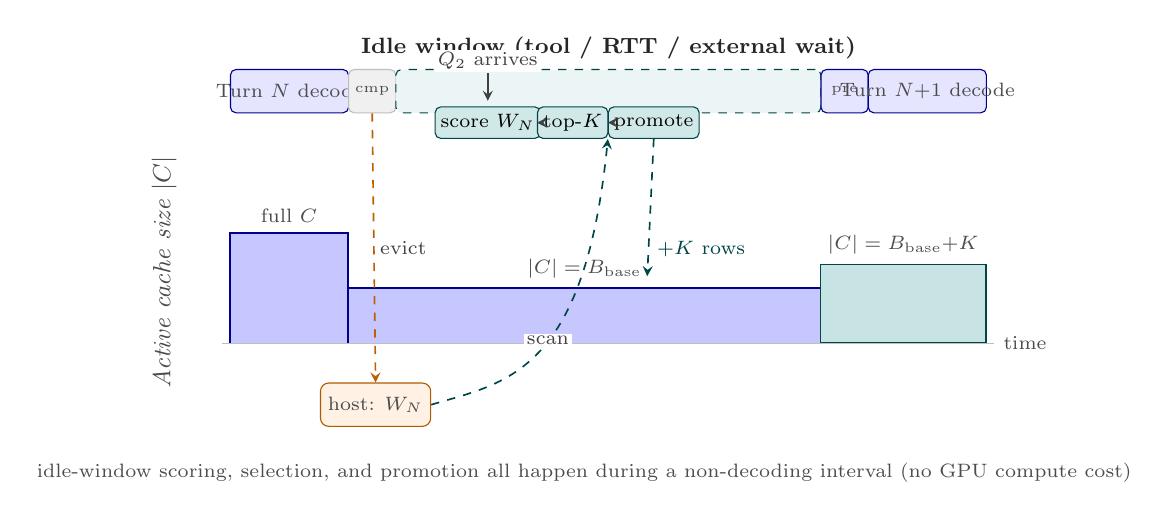
\begin{tikzpicture}[
  >=latex, line width=0.5pt,
  band/.style={rounded corners=2pt},
  decodeband/.style={band, fill=blue!10, draw=blue!55!black, line width=0.4pt,
                     minimum height=0.55cm},
  compressband/.style={band, fill=gray!12, draw=gray!50, line width=0.4pt,
                       minimum height=0.55cm},
  idleband/.style={band, fill=teal!8, draw=teal!50!black, dashed,
                   line width=0.4pt, minimum height=0.55cm},
  subop/.style={band, fill=teal!18, draw=teal!55!black, line width=0.4pt,
                minimum height=0.4cm, font=\scriptsize, align=center,
                inner sep=2pt},
  axislabel/.style={font=\scriptsize, text=black!70},
  bandlabel/.style={font=\bfseries\footnotesize, text=black!85},
  size_dropped/.style={fill=blue!22, draw=blue!55!black, line width=0.45pt},
  size_promoted/.style={fill=teal!35, draw=teal!55!black, line width=0.5pt},
  arr/.style={->, line width=0.6pt, draw=black!75, >=stealth},
  arrlabel/.style={font=\scriptsize, text=black!75, fill=white, inner sep=1pt},
  callout/.style={font=\scriptsize, text=black!70, align=center}
]
  % Top: phase bar
  \node[decodeband, minimum width=1.5cm, anchor=west] (dN) at (0, 3.2) {};
  \node[axislabel] at (dN.center) {Turn $N$ decode};
  \node[compressband, minimum width=0.6cm, anchor=west] (cmp) at (1.5, 3.2) {};
  \node[axislabel] at (cmp.center) {\rotatebox{0}{\tiny cmp}};
  \node[idleband, minimum width=5.4cm, anchor=west] (idle) at (2.1, 3.2) {};
  \node[bandlabel, anchor=south] at (idle.north)
       {Idle window (tool / RTT / external wait)};
  \node[decodeband, minimum width=0.6cm, anchor=west] (pre) at (7.5, 3.2) {};
  \node[axislabel] at (pre.center) {\tiny pre};
  \node[decodeband, minimum width=1.5cm, anchor=west] (dN1) at (8.1, 3.2) {};
  \node[axislabel] at (dN1.center) {Turn $N{+}1$ decode};

  % Sub-ops inside idle
  \node[subop, minimum width=1.1cm, anchor=west] (score) at (2.6, 2.8)
       {score $W_N$};
  \node[subop, minimum width=0.7cm, anchor=west] (select) at (3.9, 2.8)
       {top-$K$};
  \node[subop, minimum width=0.85cm, anchor=west] (promote) at (4.8, 2.8)
       {promote};

  \draw[arr] (score.east) -- (select.west);
  \draw[arr] (select.east) -- (promote.west);

  % Q_2 enters score
  \draw[arr] ([yshift=12pt]score.north) -- ([yshift=2pt]score.north);
  \node[arrlabel, anchor=south] at ([yshift=12pt]score.north) {$Q_2$ arrives};

  % |C| size axis label
  \node[font=\itshape\small, text=black!70, anchor=south, rotate=90]
       at (-0.55, 0.9) {Active cache size $|C|$};

  % Size bar
  \draw[size_dropped, fill=blue!22] (0, 0) rectangle (1.5, 1.4);
  \node[axislabel, anchor=south] at (0.75, 1.4) {full $C$};
  \draw[size_dropped, fill=blue!22] (1.5, 0) rectangle (7.5, 0.7);
  \node[axislabel, anchor=south] at (4.5, 0.7) {$|C|=\bbase$};
  \draw[size_promoted, fill=teal!22] (7.5, 0) rectangle (9.6, 1.0);
  \node[axislabel, anchor=south] at (8.55, 1.0) {$|C|=\bbase{+}K$};

  % time axis
  \draw[draw=gray!50, line width=0.3pt] (-0.1, 0) -- (9.7, 0);
  \node[axislabel, anchor=west] at (9.7, 0) {time};

  % connector arrow promote -> size step
  \draw[arr, draw=teal!55!black, dashed] (promote.south) -- (5.3, 0.85);
  \node[callout, anchor=west, text=teal!55!black] at (5.3, 1.2) {$+K$ rows};

  % W_N pool box
  \node[band, draw=orange!70!black, fill=orange!10, line width=0.4pt,
        rounded corners=3pt, minimum width=1.4cm, minimum height=0.55cm,
        anchor=north] (wnpool) at (1.85, -0.5) {};
  \node[axislabel] at (wnpool.center) {host: $W_N$};
  \draw[arr, dashed, draw=orange!75!black] (cmp.south) -- (wnpool.north)
       node[arrlabel, midway, right=1pt] {evict};
  \draw[arr, dashed, draw=teal!55!black] (wnpool.east)
       .. controls (3.5, -0.5) and (4.5, -0.4) ..
       (promote.south west) node[arrlabel, pos=0.55] {scan};

  % Caption
  \node[callout, anchor=north] at (4.5, -1.4)
       {idle-window scoring, selection, and promotion all happen during a
        non-decoding interval (no GPU compute cost)};
\end{tikzpicture}
\end{document}
